\documentclass[tikz,border=8pt]{standalone}
\usepackage{amsmath}\usepackage{pgfplots}\pgfplotsset{compat=1.18}
\definecolor{ink}{HTML}{21352F}\definecolor{teal}{HTML}{087F7B}\definecolor{gold}{HTML}{C58B2A}\definecolor{rose}{HTML}{B65A62}\definecolor{blue}{HTML}{4B77A8}
\begin{document}
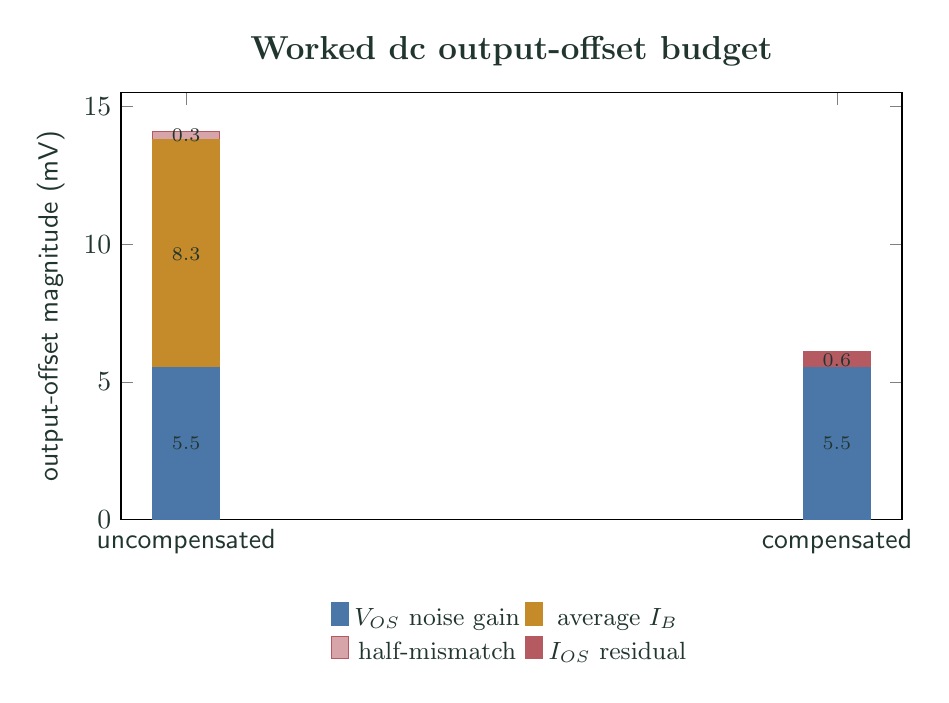
\begin{tikzpicture}[font=\sffamily,text=ink]
\begin{axis}[ybar stacked,width=11.5cm,height=7cm,bar width=24pt,ymin=0,ymax=15.5,ylabel={output-offset magnitude (mV)},symbolic x coords={uncompensated,compensated},xtick=data,legend style={draw=none,at={(.5,-.18)},anchor=north,legend columns=2,font=\small},title={Worked dc output-offset budget},title style={font=\bfseries\large},nodes near coords,nodes near coords style={font=\scriptsize}]
 \addplot[fill=blue,draw=blue] coordinates {(uncompensated,5.5)(compensated,5.5)};\addlegendentry{$V_{OS}$ noise gain}
 \addplot[fill=gold,draw=gold] coordinates {(uncompensated,8.3)(compensated,0)};\addlegendentry{average $I_B$}
 \addplot[fill=rose!55,draw=rose] coordinates {(uncompensated,.3)(compensated,0)};\addlegendentry{half-mismatch}
 \addplot[fill=rose,draw=rose] coordinates {(uncompensated,0)(compensated,.6)};\addlegendentry{$I_{OS}$ residual}
\end{axis}
\end{tikzpicture}
\end{document}
